\documentclass[11pt]{article} %[12pt]

\usepackage[utf8]{inputenc}
\usepackage[T1]{fontenc}
\usepackage{lmodern}
\usepackage[english]{babel}
\usepackage{amsmath}
\usepackage{listings}
\usepackage{graphicx}
\usepackage{enumitem}
\usepackage{amssymb}
\usepackage{verbatim}
\usepackage{pdfpages}
\usepackage{algpseudocode}
\usepackage{breqn}
\usepackage[linesnumbered,ruled,vlined]{algorithm2e}
\usepackage{tikz}
\usetikzlibrary{positioning,shapes.multipart}
\usepackage{textcomp}
\SetArgSty{textup}
\usepackage{fancyhdr}

\topmargin -2cm 
\textheight 24cm
\textwidth 16.0 cm 
\oddsidemargin -0.1cm

 
 \pagestyle{fancy}
 \fancyhf{}
 \fancyhead[LE,RO]{Exercise 2}
 \fancyhead[RE,LO]{Deep Learning for Computer Vision}
 \fancyfoot[CE,CO]{\leftmark}
 \fancyfoot[LE,RO]{\thepage}

\newcommand{\R}{\mathbb{R}}
\newcommand{\E}{\mathbb{E}}
\newcommand{\Var}{\mathrm{Var}}
\newcommand{\N}{\mathbb{N}}
\newcommand{\Q}{\mathbb{Q}}
\newcommand{\C}{\mathbb{C}}
\newcommand{\Z}{\mathbb{Z}}
\newcommand{\ggT}{\text{ggT}}
\newcommand{\kgV}{\text{kgV}}
\newcommand{\spa}[1]{\; #1 \;}
\newcommand{\bewbeh}[2]{\begin{enumerate} \item[\textbf{Beh.}]#1 \item[\textbf{Bew.}]#2
	\end{enumerate}}
\newcommand{\induct}[2]{\begin{enumerate} \item[\textit{IA}]#1 \item[\textit{IS}]#2
	\end{enumerate}}
\newcommand{\qed}{\hfill\ensuremath{\square}}
\newcommand{\gdw}[2]{\begin{enumerate} \item[$\Rightarrow$]#1 \item[$\Leftarrow$]#2
	\end{enumerate}}
\newcommand{\intsto}[1]{\{1, \dots, #1\}}
\newcommand\Item[1][]{%
	\ifx\relax#1\relax  \item \else \item[#1] \fi
	\abovedisplayskip=0pt\abovedisplayshortskip=0pt~\vspace*{-\baselineskip}}



\begin{document}
\section*{Exercise 2.1 c}
\begin{figure}[htb]
  \centering
  \centerline{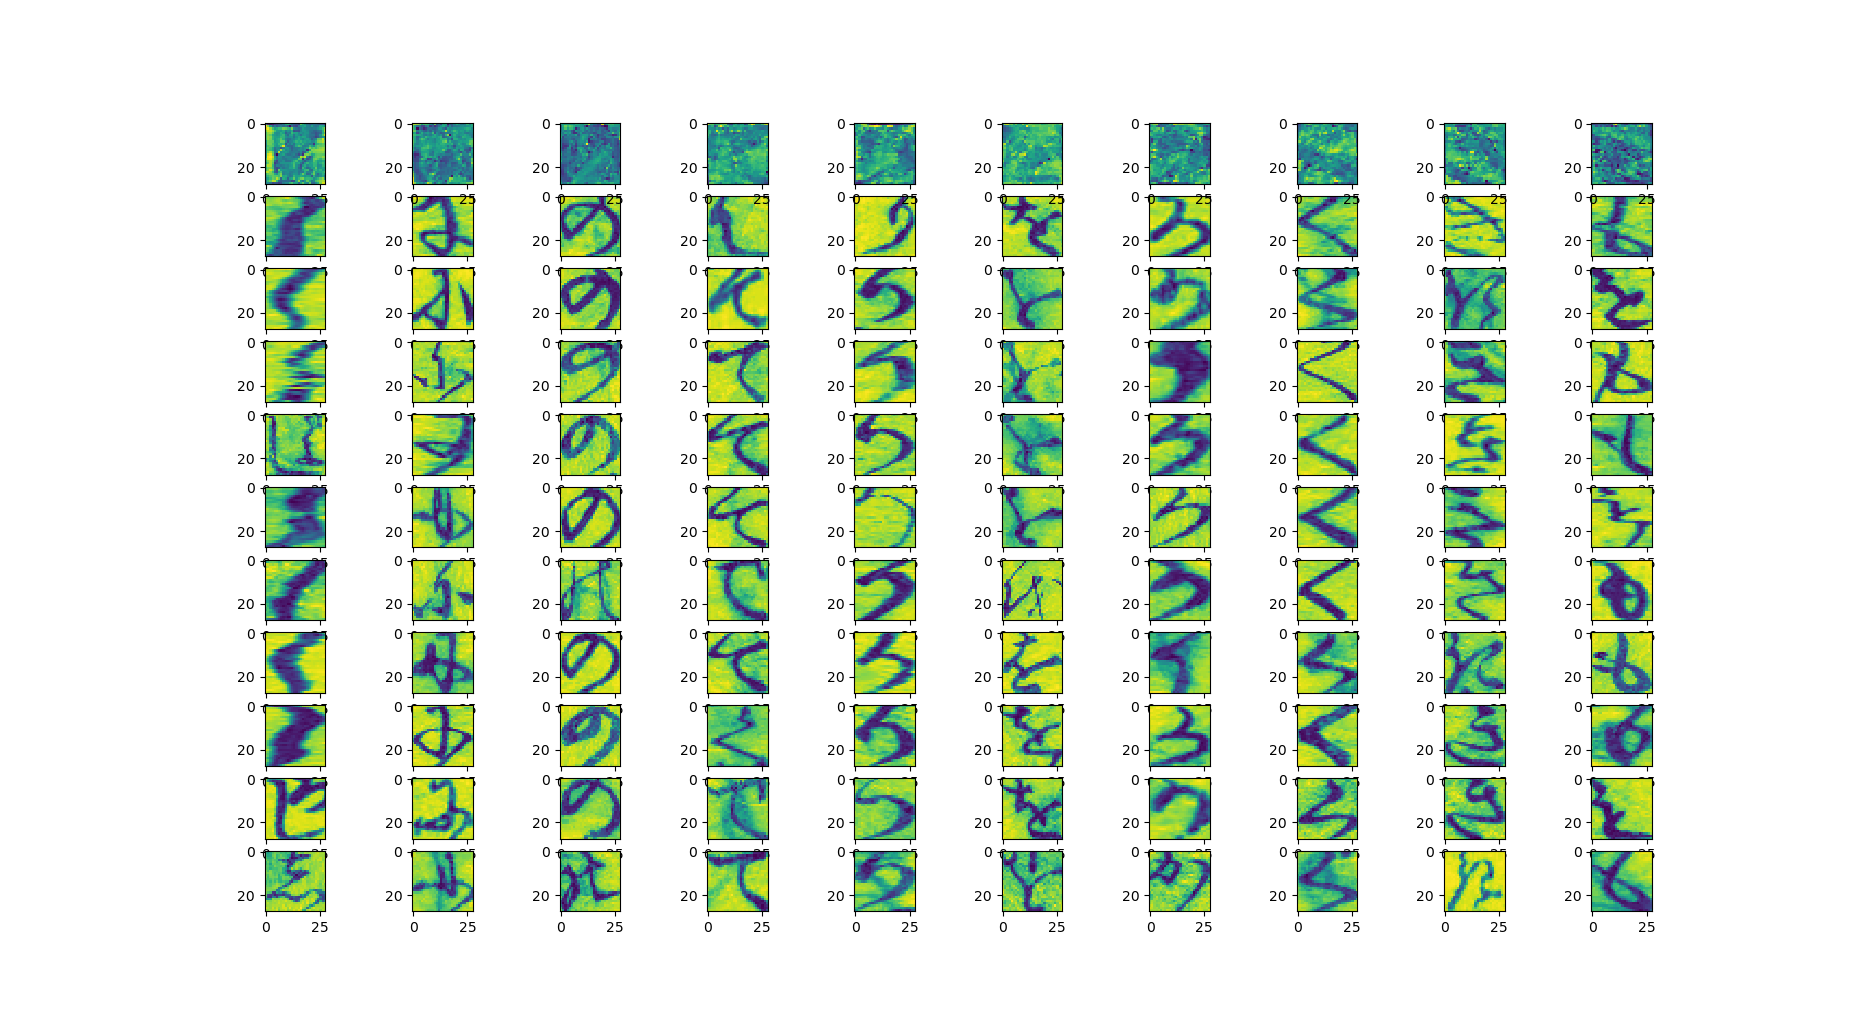
\includegraphics[width=1.35\textwidth ]{Figure_1_1.png}}
  \vspace{-5pt}
    \centering
\caption{Visualization of the weights vectors and example data images. The darker parts in the visualization of the weights vectors look similar to the real example images.}
\vspace{-1pt}
\end{figure}
\clearpage

\section*{Exercise 2.2}
\begin{figure}[htb]
  \centering
  \centerline{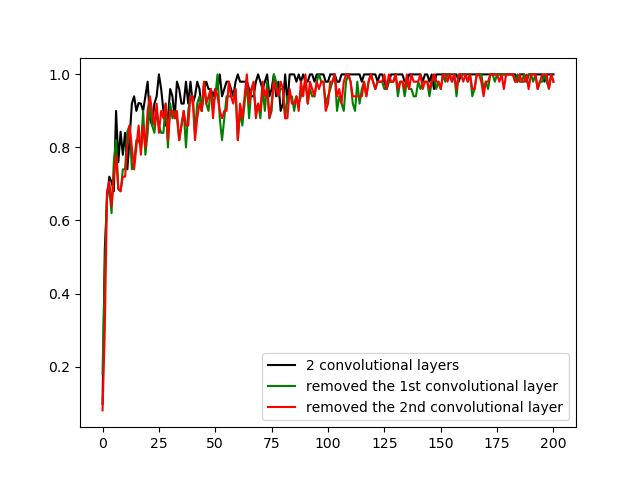
\includegraphics[width=0.6\textwidth ]{Figure_2_4.png}}
  \vspace{-5pt}
    \centering
\caption{(c). Visualization of training accuracies while removing convolutional layers}
\vspace{-1pt}
\end{figure}

\begin{figure}[htb]
  \centering
  \centerline{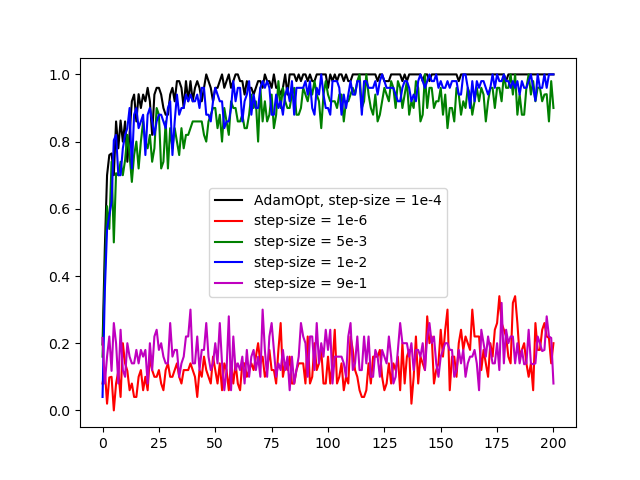
\includegraphics[width=0.6\textwidth ]{Figure_2_5.png}}
  \vspace{-5pt}
    \centering
\caption{(d). Visualization of training accuracies with changing the step size. Too small step size will make the gradient descent progress so slowly that within the iterations it cannot reach or come out of a local minimum; Too large step size will make the gradient descent travel between two sides of a (local) minimum and never reach it.}
\vspace{-1pt}
\end{figure}
\clearpage

\section*{Exercise 2.3}

\begin{figure}[htb]
  \centering
  \centerline{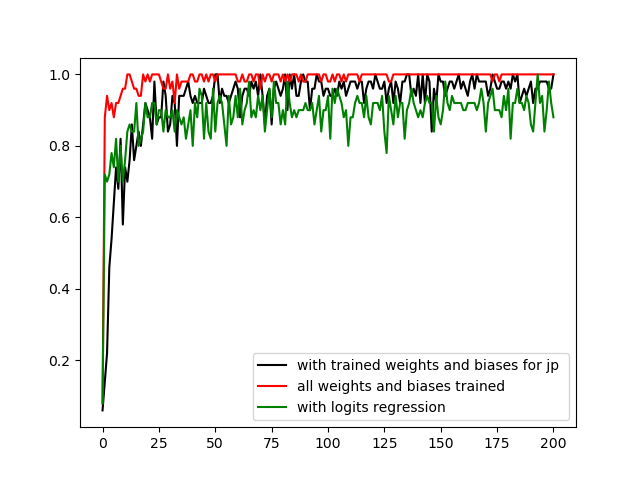
\includegraphics[width=1\textwidth ]{Figure_3.png}}
  \vspace{-5pt}
    \centering
\caption{Visualization of training MNIST with different strategies.}
\vspace{-1pt}
\end{figure}
\clearpage

\section*{Exercise 2.5}
\begin{enumerate}[label= (\alph*) \;]
  \item $ \displaystyle
    \E(\bar x) = \E\Big( \frac 1 L \sum_{l=1}^L x_l \Big)
    = \frac 1 L \sum_{l=1}^L \E(x_l)
    = \frac 1 L \sum_{l=1}^L \frac \theta 2
    = \frac \theta 2$

  \item With $\hat x := 2 \bar x$ it is
    $\E(\hat x) = \E(2 \bar x) = 2 \E(\bar x) = \theta$.

  \item The standard error
    \[ \displaystyle
      \E((\hat x - \theta)^2)
      = \E((\hat x - \E(\hat x))^2)
      = \Var(\hat x)
      = \Var\Big( \frac 2 n \sum_{l=1}^L x_l \Big)
      = \frac{4}{L^2} \sum_{l=1}^L \Var(x_l)
      = \frac 4 L \Var(x_1)
    \]
    clearly goes to zero for $L \to \infty$.

  \item Let $\tilde x := \hat x + \frac 1 L$. It is
    \[
      \E(\tilde x)
      = \E(\hat x + \frac 1 L)
      = \theta + \frac 1 L
    \]
    and
    \[
      \E((\tilde x - \theta)^2)
      = \E((\hat x + \frac 1 L - \theta)^2)
      = \E((\hat x - \theta)^2 + \frac{1}{L^2} + \frac 2 L (\hat x - \theta))
      = \frac 4 L \Var(x_1) + \frac{1}{L^2}
    \]
    which goes to zero for $L \to \infty$.
\end{enumerate}

\end{document}
